%% All authors must submit their articles at
%% \href{http://www.pnascentral.org/cgi-bin/main.plex}{PNAScentral}. If
%% you are using Overleaf to write your article, you can use the ``Submit
%% to PNAS'' option in the top bar of the editor window.

\documentclass[9pt,twocolumn,twoside,lineno]{pnas-new}
% Use the lineno option to display guide line numbers if required.

\templatetype{pnasresearcharticle} % Choose template 
% {pnasresearcharticle} = Template for a two-column research article
% {pnasmathematics} %= Template for a one-column mathematics article
% {pnasinvited} %= Template for a PNAS invited submission

\title{Genotypic variation in a foundation tree directs ecological
  network structure}

% Use letters for affiliations, numbers to show equal authorship (if
% applicable) and to indicate the corresponding author

\author[a,b,1]{Matthew K. Lau}
\author[b]{Louis J. Lamit}
\author[c]{Rikke R. Naesbourg}
\author[d]{Stuart R. Borrett}
\author[e]{Matthew A. Bowker}
\author[a]{Thomas G. Whitham}

%% Include department, institution, and complete address, with the
%% ZIP/postal code, for each author. Use lower case letters to match
%% authors with institutions, as shown in the example. 
%% Authors with an ORCID ID may supply this information at submission.

\affil[a]{Department of Biological Sciences and Merriam-Powell Center
  for Environmental Research, Northern Arizona University, Flagstaff,
  AZ 86011, USA}
\affil[b]{Harvard Forest, Harvard University, 324 N Main St,
  Petersham, MA 01366, USA}
\affil[c]{University of California Berkeley, Berkeley, CA, USA}
\affil[d]{Department of Biology and Marine Biology, University of
  North Carolina Wilmington, 601 South College Road, Wilmington, NC, 28403, USA}
\affil[e]{School of Forestry, Northern Arizona University, Flagstaff, AZ 86011, USA}

% Please give the surname of the lead author for the running footer
\leadauthor{Lau} 
% Use letters for affiliations, numbers to show equal authorship (if
% applicable) and to indicate the corresponding author
% Please add here a significance statement to explain the relevance of your work

\significancestatement{Authors must submit a 120-word maximum
  statement about the significance of their research paper written at
  a level understandable to an undergraduate educated scientist
  outside their field of speciality. The primary goal of the
  Significance Statement is to explain the relevance of the work in
  broad context to a broad readership. The Significance Statement
  appears in the paper itself and is required for all research
  papers.}

% Please include corresponding author, author contribution and author declaration information

\authorcontributions{M.L. and L.L. conceived the study, M.L. and
  L.L. conducted the field work, R.N.  assisted in lichen
  identifications, M.L. wrote the first draft of the manuscript,
  S.B. and T.W. contributed substantively to the conceptual
  development, T.W. established the common garden. All authors
  contributed to revisions of the manuscript.}
\authordeclaration{The authors have no conflicts of interest.}
\correspondingauthor{\textsuperscript{1}Dr. Matthew K. Lau. E-mail: matthewklau@fas.harvard.edu}

% Keywords are not mandatory, but authors are strongly encouraged to
% provide them. If provided, please include two to five keywords,
% separated by the pipe symbol, e.g:
\keywords{Keyword 1 $|$ Keyword 2 $|$ Keyword 3 $|$ ...} 

\begin{abstract}
%% Please provide an abstract of no more than 250 words in a single
%% paragraph. Abstracts should explain to the general reader the major
%% contributions of the article. References in the abstract must be
%% cited in full within the abstract itself and cited in the text.

%% Currently: 272 words 13Dec2018

Biological evolution occurs in the context of complex networks of
interacting species in which natural selection defines the structure
of ecological networks. Fundamental to this evolutionary process is
the discovery of a genetic basis to ecological network
structure. Although previous work has demonstrated that tree genotype
contributes to interaction network structure at the scale of forest
stands, the contribution of tree genetics to localized interaction
networks at the scale of individual trees has not yet been
explored. To test the degree to which tree genetics can contribute to
network structure, we conducted quantitative modeling of interaction
network for a community of epiphytic lichens in a long-term
experimental common garden of genotyped trees of a foundation species
(\textit{Populus angustifolia}). We found three main results: 1) bark
roughness and lichen communities displayed signficant responses to
tree genotype, 2) tree genotype strongly contributed to network
structure, explaining a third of the variation in lichen interaction
networks, and 3) several metrics of interaction network structure
varied in response to genotype, including the number of interactions
and centralization. These results support the hypothesis that
variation in ecological interaction networks can result from
genetically based variation in foundation species. This study opens
the possibility for a genetic basis to both direct and indirect
interactions among species in complex communities.

\end{abstract}

\dates{This manuscript was compiled on \today}
\doi{\url{www.pnas.org/cgi/doi/10.1073/pnas.XXXXXXXXXX}}

\begin{document}

%% Many authors find it useful to organize their manuscripts with the
%% following order of sections; Title, Author Affiliation, Keywords,
%% Abstract, Significance Statement, Results, Discussion, Materials
%% and methods, Acknowledgments, and References. Other orders and
%% headings are permitted.

%% PNAS generally uses a two-column format averaging 67 characters,
%% including spaces, per line. The maximum length of a Direct
%% Submission research article is six pages and a Direct Submission
%% Plus research article is ten pages including all text, spaces, and
%% the number of characters displaced by figures, tables, and
%% equations.  When submitting tables, figures, and/or equations in
%% addition to text, keep the text for your manuscript under 39,000
%% characters (including spaces) for Direct Submissions and 72,000
%% characters (including spaces) for Direct Submission Plus.

%% Authors may use 1- or 2-column equations in their article,
%% according to their preference.

%% To allow an equation to span both columns, use the
%% \verb|\begin{figure*}...\end{figure*}| environment mentioned above
%% for figures.

%% Note that the use of the \verb|widetext| environment for equations
%% is not recommended, and should not be used.

%% \begin{figure*}[bt!]
%% \begin{align*}
%% (x+y)^3&=(x+y)(x+y)^2\\
%%        &=(x+y)(x^2+2xy+y^2) \numberthis \label{eqn:example} \\
%%        &=x^3+3x^2y+3xy^3+x^3. 
%% \end{align*}
%% \end{figure*}


%% \begin{table}%[tbhp]
%% \centering
%% \caption{Comparison of the fitted potential energy surfaces and ab initio benchmark electronic energy calculations}
%% \begin{tabular}{lrrr}
%% Species & CBS & CV & G3 \\
%% \midrule
%% 1. Acetaldehyde & 0.0 & 0.0 & 0.0 \\
%% 2. Vinyl alcohol & 9.1 & 9.6 & 13.5 \\
%% 3. Hydroxyethylidene & 50.8 & 51.2 & 54.0\\
%% \bottomrule
%% \end{tabular}

%% \addtabletext{nomenclature for the TSs refers to the numbered species in the table.}
%% \end{table}

%% References should be cited in numerical order as they appear in
%% text; this will be done automatically via bibtex,
%% e.g. \cite{belkin2002using} and
%% \cite{berard1994embedding,coifman2005geometric}. All references
%% should be included in the main manuscript file.

%% PNAS must be able to archive the data essential to a published
%% article. Where such archiving is not possible, deposition of data
%% in public databases, such as GenBank, ArrayExpress, Protein Data
%% Bank, Unidata, and others outlined in the Information for Authors,
%% is acceptable.


%% Only TIFF, EPS, and high-resolution PDF for Mac or PC are allowed
%% for figures that will appear in the main text, and images must be
%% final size. Authors may submit U3D or PRC files for 3D images;
%% these must be accompanied by 2D representations in TIFF, EPS, or
%% high-resolution PDF format.  Color images must be in RGB (red,
%% green, blue) mode. Include the font files for any text.

%% Figures and Tables should be labelled and referenced in the
%% standard way using the \verb|\label{}| and \verb|\ref{}| commands.

%% Figure \ref{fig:frog} shows an example of how to insert a
%% column-wide figure. To insert a figure wider than one column,
%% please use the \verb|\begin{figure*}...\end{figure*}|
%% environment. Figures wider than one column should be sized to 11.4
%% cm or 17.8 cm wide. Use \verb|\begin{SCfigure*}...\end{SCfigure*}|
%% for a wide figure with side captions.

%% Authors should submit SI as a single separate PDF file, combining
%% all text, figures, tables, movie legends, and SI references.  PNAS
%% will publish SI uncomposed, as the authors have provided it.
%% Additional details can be found here:
%% \href{http://www.pnas.org/page/authors/journal-policies}{policy on
%% SI}.  For SI formatting instructions click
%% \href{https://www.pnascentral.org/cgi-bin/main.plex?form_type=display_auth_si_instructions}{here}.
%% The PNAS Overleaf SI template can be found
%% \href{https://www.overleaf.com/latex/templates/pnas-template-for-supplementary-information/wqfsfqwyjtsd}{here}.
%% Refer to the SI Appendix in the manuscript at an appropriate point
%% in the text. Number supporting figures and tables starting with S1,
%% S2, etc.

%% Authors who place detailed materials and methods in an SI Appendix
%% must provide sufficient detail in the main text methods to enable a
%% reader to follow the logic of the procedures and results and also
%% must reference the SI methods. If a paper is fundamentally a study
%% of a new method or technique, then the methods must be described
%% completely in the main text.


\maketitle
\thispagestyle{firststyle}
\ifthenelse{\boolean{shortarticle}}{\ifthenelse{\boolean{singlecolumn}}{\abscontentformatted}{\abscontent}}{}

% If your first paragraph (i.e. with the \dropcap) contains a list
% environment (quote, quotation, theorem, definition, enumerate,
% itemize...), the line after the list may have some extra
% indentation. If this is the case, add \parshape=0 to the end of the
% list environment.

%% \dropcap{T}his PNAS journal template is provided to help you write
%% your work in the correct journal format.  Instructions for use are
%% provided below.

%% Note: please start your introduction without including the word
%% ``Introduction'' as a section heading (except for math articles in
%% the Physical Sciences section); this heading is implied in the
%% first paragraphs.

\dropcap{E}volution occurs in the context of complex networks of
interacting species. In ecological communities, community dynamics
depend on key interactions \cite{Fontaine2011} that occur in species
interaction networks, such as:  trophic \cite{Bascompte2006} and
mutualistic \cite{Rafferty2013} interaction networks. Phylogenetic
patterns in ecological networks support the importance of evolutionary
processes in shaping species interactions, community structure and
ecosystem processes \cite{Crutsinger2016, Rezende2007, Whitham2006a}. 

More on ecological networks 

Community genetics studies \cite{Lamit2015} have shown that
genetic variation in foundation species \cite{Ellison2005} plays a
significant role in defining distinct communities of interacting
organisms:  such as, endophytes, pathogens, lichens, arthropods, and
soil microbes. Multiple studies have now demonstrated that genetic
variation influences numerous functional traits (e.g., phytochemical,
phenological, morphological) produces a multivariate phenotype
\cite{holeski2012} tha contributes to variation in associated
communities \cite{Bailey2009a}.

Additional work has provided support for the hypothesis that not only
does composition vary among genetically distinct genotypes of
foundation species but it also impacts the structure of the network of
species interactions in these communities \cite{Keith2017,
  Lau2016}. Also, work by \citep{Toju2018, Toju2015, Toju2014}
observed consistent patterns of centralized interactions of species
modules focused around hubs of plant-fungal interactions. In other
words, a small number of plant and fungal symbionts tended to have
have disproportionate numbers of interactions with other species and
likely are the drivers in determining community assembly, structure
and dynamics.

Here, we investigate how genetic variation in a foundation tree
species determines the structure of a network of interactions among a
community of tree associated lichen species. Using a long-term (20+
years), common garden experiment with replicated individuals of known
genetic identity and a naturally established stand of \textit{Populus
  angustifolia}. We focused on a model community of 9 epiphytic
lichens species, as previous research has demonstrated significant
compositional responses of epiphytes to genotypic variation
\cite{Winfree2011, Zytynska2011}. In addition, the life-history
characteristics of lichen, having highly localized, direct contact
interactions and slow population turnover rates, allowed us to assess
interactions among lichen species on individual trees. We hypothesize
that in natural systems evolution occurs in a community context
involving interactions of complex networks of interacting species
\cite{Lau2016, Keith2017, Thompson2013, Bascompte2007, Darwin1855}.
If correct, we should expect to find that network structure is
genetically based in which different plant genotypes support different
interaction networks and that these interactions networks can function
as indicators of ecological dynamics important for conserving
biodiversity.  Applying a probability-theory based network modeling
approach, we constructed a set of interaction network models for the
lichen associated with individual trees. Using these models, we then
examined the genetic basis a foundation tree species on the structure
of ecological networks.

\matmethods{


The study was conducted along the Weber River, UT (USA), which is a
cottonwood (\textit{Populus} spp.) dominated riparian
ecosystem. Although two native species, \textit{Populus angustifolia}
(James) and \textit{Populus fremontii} (S. Watson), occur here and are
known to hybridize, only pure or advanced generation backcrosses of
\textit{P. angustifolia} were sampled in order to avoid the effect of
the hybridization between these two species \cite{Zinkgraf2016}.

A common garden was used to isolate the effect of tree genotype from
the effect of the localized microenvironment associated with each
individual and spatial autocorrelation. Asexually propagated clones of
genotyped \textit{P. angustifolia} individuals were obtained from wild
collections and planted randomly in a single field (0.025 km$^2$) at
the Ogden Nature Center, Ogden, UT in 1992. A total of thirteen
genotypes replicated between 3 and 8 times each, were chosen for
sampling. Genotype names were previously published in
\citep{Martinsen}.


\subsection*{Bark Lichen Observations}

On each tree, presence or absence of each lichen species was assessed
in 50 total 1 cm$^2$ cells arrayed in a checkerboard pattern. Given
the small size and sessile nature of lichen, we were able to rapidly
assess lichen interactions by quantifying thalli in close
contact. Sampling was restricted to the northern aspect of the trunk
to maximize the abundance of lichen and control for the effect of
trunk aspect. Two adjacent 10 cm$^2$ quadrats centered at 50 cm and 85
cm from ground level were sampled (Fig~\ref{fig:lichen_sampling} A and
B). The bark lichen community in this system is comprised of fourteen
species; however, only 9 species were observed within our study
quadrats (Fig~\ref{fig:lichen_sampling} C-K). The observed lichen
community included (abbreviations are given for species present in
study): Xg = \textit{Xanthomendoza galericulata}, Xm =
\textit{X. montana}, Ch = \textit{Caloplaca holocarpa}, Cs =
\textit{Candelariella subdeflexa}, Rg = \textit{Rinodina glauca}, Lh =
\textit{Lecanora hagenii}, Ls = \textit{Lecanora} sp., Pm =
\textit{Phyciella melanchra}, Pa = \textit{Physcia adscendens}, Pu =
\textit{Physcia undulata}. Several other species were not obesrved in
the present study but are known to occur in this region:
\textit{Phaeophyscia orbicularis}, \textit{Phaeophyscia ciliata},
\textit{Melanelia subolivacea}, \textit{Meanelia elegantula}. Species
accumulation curves indicated that communities in the the common
garden were thoroughly sampled and similar in composition and richness
to nearby naturally established cottonwood stands (Supplementary
Materials).

The cell size and checkerboard sampling pattern was chosen to isolate
the individuals in each cell. In a previous survey of lichen thallus
size in this common garden, we had observed a median thallus size of
0.12 $\pm$ 0.001 cm$^2$ (S.E.) \cite{Lamit2015}. Based on this, we
expected thalli observed in each cell to generally be spatially
independent of the other cells in the quadrat but exposed to similar
micro-environmental conditions created by the bark and the location of
the sampling area on an individual tree. Therefore, we were confident
in treating the cell-wise observations in quadrats as independent with
respect to lichen-lichen interactions.

As bark roughness had previously been shown to be an important,
genetically based tree trait impacting bark lichen, we measured the
percentage of rough bark on each tree following the methods of
\citep{Lamit2012}. Briefly, the number of cells containing disrupted,
fissured bark were counted within each quadrat on each tree. The
number of rough bark containing cells were then summed and divided by
the total number of cells surveyed. This was done for all quadrats on
all trees in which lichen communities were also observed.


\begin{figure}[ht]
\centering
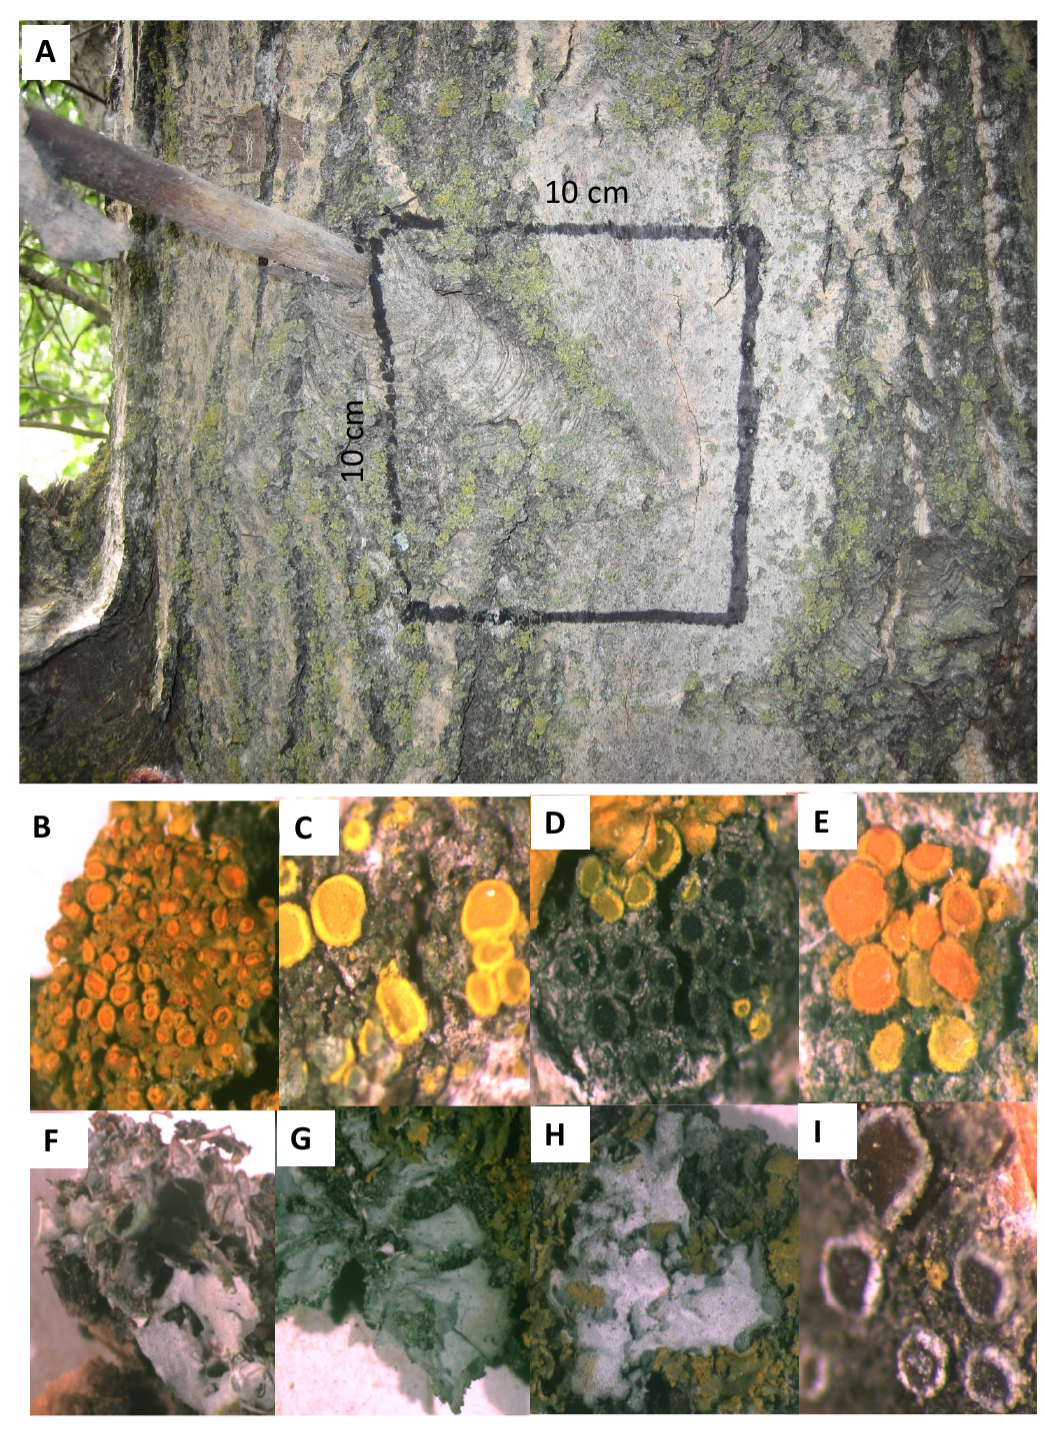
\includegraphics[width=\linewidth]{lcn_sampling.pdf}
\caption{The communities of bark lichen were observed in a common
  garden of replicated genotypes of narrowleaf cottonwood trees
  (\textit{P. angustifolia}) at the Ogden Nature Center (Ogden,
  UT). Lichen were sampled within a fixed area (10cm by 10cm) on
  individual trees (A and B). (C) a photo of a typical community of
  bark lichen species interacting on the trunk of a cottonwood tree,
  including one of the more abundant species, \textit{Xanthomendoza
    galericulata}, in the center. (D-K) shows the other main lichen
  species observed, respectivley:  \textit{X. montana},
  \textit{Candelariella subdeflexa}, \textit{Rinodina} sp.,
  \textit{Caloplaca holocarpa}, \textit{Physcia adscendens},
  \textit{Phyciella melanchra}, \textit{Physcia undulata} and
  \textit{Lecanora hageni}.}
\label{fig:lichen_sampling}
\end{figure}



\subsection*{Lichen Network Modeling and Analysis}

We used the observations of lichen in the 1cm2 cells on individual
trees of \textit{P. angustifolia}. Unipartite networks were generated
using the conditional probabilities of each species pair, i.e. the
probability of observing one species given an observation of another
species $P(S_i | S_j)$, based on the method developed by
\citep{Araujo2011}. To calculate conditional probabilities, we
quantified the individual probabilities of species occurrences
$P(S_i)$ and the joint probability of co-occurrences $P(S_i,S_j)$
using the frequencies of each species and their co-occurrences. We
were then able to calculate the conditional probabilities of each
species pair as $P(S_i|S_j) = \frac{P(S_i,S_j)}{P(S_j)}$, based on the
axioms of probability. This yielded an asymetric matrix, that is
$P(S_i|S_j)$ does not have to be equal to $P(S_j|S_i)$, that also had
a diagonal $S_{ii}$ equal to one for all species present and zero for
species that were not observed on the tree.

We then applied an analytical procedure to remove non-significant
links between species. This procedure determines if the joint
probability of a species pair (i.e. $P(S_i,S_j)$) is different from
zero (Fig.~\ref{fig:conet_method}).  Here, a confidence interval
$CI_{95\%}$ is calculated as as $CI_{95\%} = E[S_iS_j] * Z_{95\%} *
\sqrt{V(S_iS_j)}$, where the expected frequency of co-occurrences
E($S_iS_j$) is the total number of cells surveyed ($N$) times the
independent probabilities of each species $P(S_i) * P(S_j)$,
$Z_{95\%}$ is the Z-score for 95\% from a Z-distribution and the
expected variance of $E(S_iS_j)$ is the total number of cells times
the expected probability of $S_iS_j$ and its compliment
(i.e. $V(S_iS_j) = N * E[P(S_i,S_j)] * (1 - E[P(S_i,S_j)])$). If the
observed number of co-occurrence falls outside of the confidence
interval, the joint probability $P(S_i,S_j)$ is determined to be equal
to the product of the individual probabilities (i.e. $P(S_i) \dot
P(S_j)$), and the conditional probability reduces to the individual
probability of that species $P(S_i)$. Therefore, unless the
co-occurrence of a species pair falls outside the confidence interval,
the probability that the observation of one species given the other is
no different than simply observing that species alone. This enables us
to remove links from a given network by re-scaling the resulting
conditional probabilities by subtracting the individual probabilities
from the conditional probabilities (i.e. how different the conditional
probability is from the independent probability), which makes any
species with a non-signficant conditional probability zero. The
resulting matrix ($\mathbf{D} = D_{ij}$) can be interpreted as how one
species impacts another with zero being no effect and values less than
or greater than zero interpreted as negative and positive effects,
respectively. Here, we will refer to this matrix ($\mathbf{D}$) as an
interaction matrix with the properties that it can be assymetric
(i.e. $P_{ij}$ does not necessarily equal $P_{ji}$), and the diagonal
($P_{ii}$) is zero (i.e. a species does not influence it's own
probability of being observed).

\begin{figure}[ht]
\centering
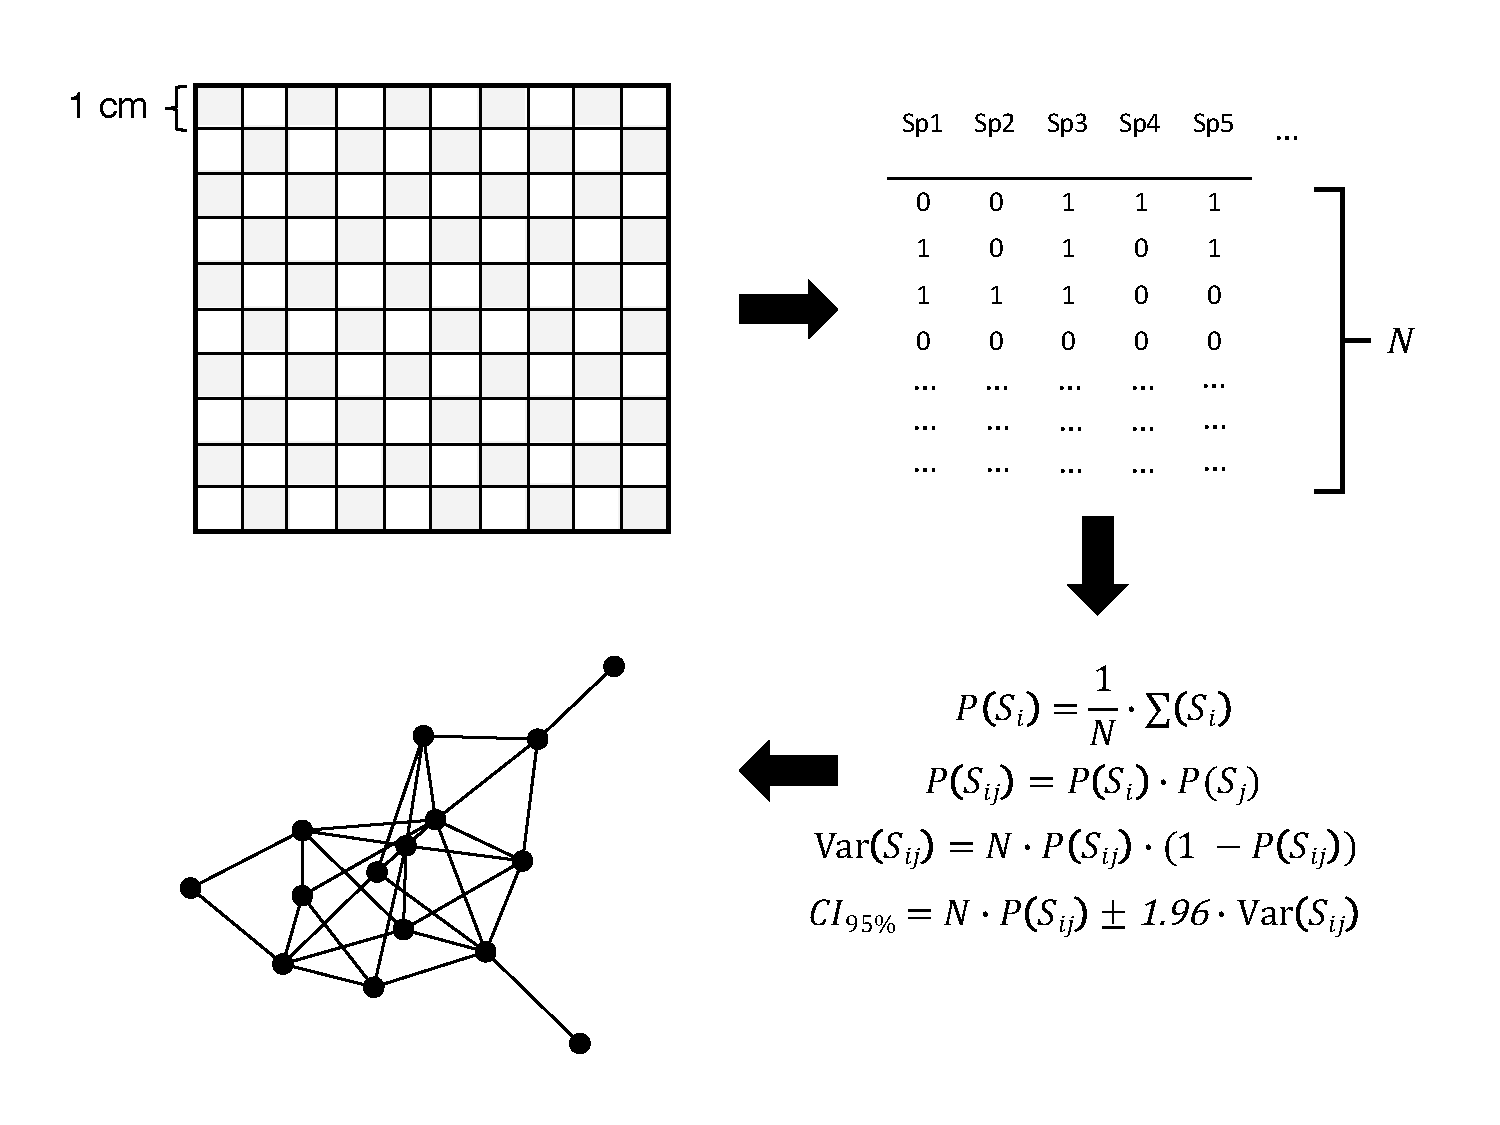
\includegraphics[width=\linewidth]{lcn_araujo_method.pdf}
\caption{Lichen interaction networks were constructed by conducting
  field observations in 1 cm$^2$ cells within a 10 cm$^2$ grid on each
  tree using a checkerboard pattern (grey cells). Thus, a set of $N$
  total cell observations were recorded for each tree with the
  presence or absence of each species recorded for each cell. Applying
  the probability-based network modeling method adapted from
  \cite{Araujo2011}, we calculated the conditional probabilities,
  $P(S_i|S_j)$, for all species pairs and removed (i.e. set equal to
  zero) species pairs whose joint probabilities, $P(S_i S_j)$, were
  not significant using a confidence interval based comparison of
  their observed co-occurrence frequency, $S_iS_j$, to that expected
  due to chance alone, $E[P(S_iS_j)] = P(S_i) P(S_j)$, and
  $P(S_i|S_j)$ reduces to $P(S_i)$, the observed individual
  probability of species $S_i$.}
\label{fig:conet_method}
\end{figure}



\subsection*{Statistical Analyses, Software and Data}

We used a combination of parametric and non-parametric, permutation
based frequentist statistical analyses to test for the effects of
genetic variation on lichen communities and their interaction
networks. To assess the effect of genotype on univariate responses, we
used random effects models with Restricted Maximum Likelihood
(REML). We used a combination of Least Squares Regression, Analysis of
Variance (ANOVA) and correlation tests to quantify and test for the
relationship among other variables. For multivariate response
variables, such as lichen community composition and network structure,
we used distance based multivariate statistical approaches, including
Permutational Analysis of Variance (PerMANOVA) and Mantel tests. For
visualization purposes, we also used Non-metric Multi-Dimensional
Scaling (NMDS) \cite{ecodist} to produce dimensionally reduced
ordinations of these multi-variate responses and fitted vectors for
continuous predictor variables to the ordinated values
\cite{vegan}. For community composition we used Bray-Curtis
dissimilarity, which has optimal performace with count data
\citep{Minchen1998}. To quantify the similarity of lichen networks
among individual trees, we calculated the pairwise Euclidean distance
of the $\mathbf{D}$ interaction matrices among all pairs of trees.


For each network, we also calculated two network metrics that measure
different structural aspects. We calculated the number of interactions
or ``links'' in each network, which provides a measure of the size of
the network \citep{Lau2014, Borrett2015}. We also calculated the
centralization of each network, which measures the evenness of the
distribution of interactions among the species in the network
\cite{Butts2005}. In a network with a low level of centralization
species have similar amount of interaction in the network, while a
network with a high level of centralization tends to one or small
subset of species that interact with other species. We used a related
function to calculate the centrality of each species in each network
as well. Although there are many other metrics, see \citep{Lau2016},
we focus on a subset for the sake of simplicity and because some
metrics are not appropriate for our relatively small communities. In
particular, we do not present analysis of the modularity (i.e. the
degree of sub-grouping) because our community has relatively few
species to form modules.

We have made all code and data available online. Code is available at
\url{github.com/communitygenetics/lcn}. Data is available via the
Harvard Dataverse (needs project ID). The project is also archived via
Zenodo at \url{zenodo.com/doiXXXXXX}. All analyses were conducted
using the programming language R version 3.4.2 (R Development Core
Team 2018).

\section*{Results}

%%% This subsection analyzes the respones of the
%%% bark lichen community to tree genotype 

\begin{figure}[ht]
\centering
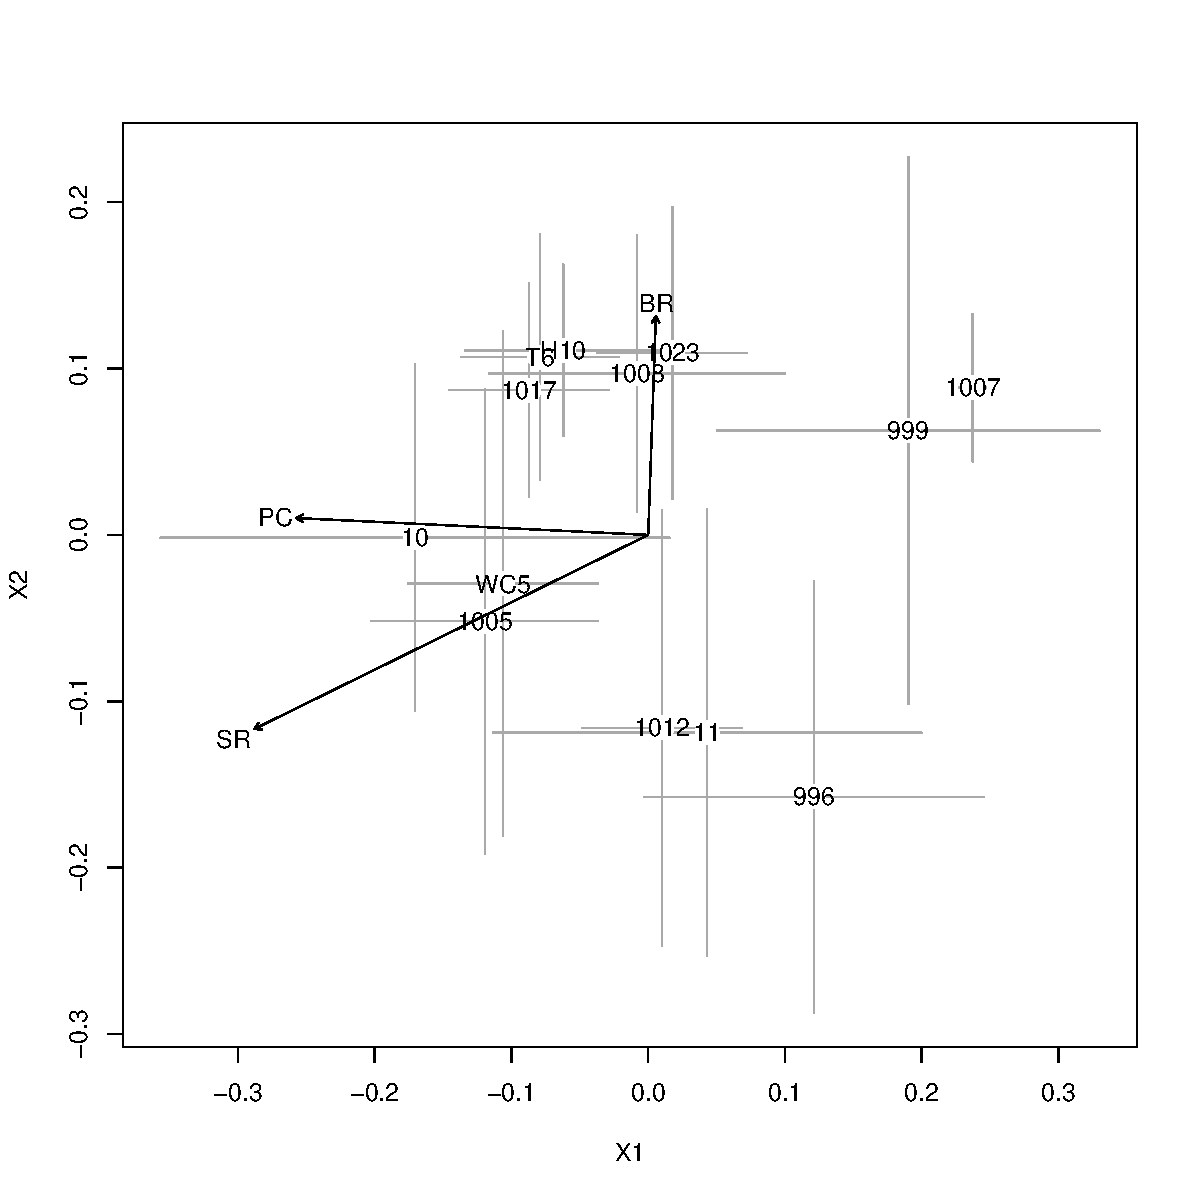
\includegraphics[width=\linewidth]{com_chplot_onc.pdf}
\caption{Lichen community composition varied among genotypes. Plot of
  the ordinated centroids ($\pm$ 1 S.E.) from the NMDS ordinated
  community composition of each genotype (indicated by centroid
  labels). Centroids that are closer together have more similar lichen
  communities.}
\label{fig:com_ch_plot}
\end{figure}


Bark roughness and some lichen community characteristics responded to
tree genotype. Percent rough bark varied signficantly among genotypes
(REML $R^2$ = ?, RLRT = 10.69, p-value = 3e-04), as did total lichen
cover (REML $R^2$ = ?, RLRT = 2.9627, p-value = 0.0375) and community
composition (PerMANOVA $R^2$ = 0.243, F 12 = 1.8221, p-value =
0.0029). However, lichen species richness did not show a significant
response to genotype (REML RLRT = 0.13047, p-value =
0.3134). Community composition was correlated with lichen cover
(PerMANOVA $R^2$ = 0.236, $F_1$ = 21.2661, p-value = 9.999e-05) and
richness (PerMANOVA $R^2$ = 0.054, $F_1$ = 4.9036, p-value = 0.0011)
after controlling for tree genotype effects
(Fig.~\ref{fig:com_ch_plot}). Roughness did not predict community
composition (PerMANOVA $R^2$ = 0.011, F 1 = 0.9938, p-value = 0.3841)
even though it was correlated with total lichen cover (ANOVA
$F_{1,55}$ = 6.797, p-value = 0.01173). Roughness was not correlated
with lichen species richness (ANOVA $F_{1, 55}$ = 1.509, p-value =
0.2246).


\subsection*{Tree genotype influenced lichen network similarity}

\begin{figure}[ht]
\centering
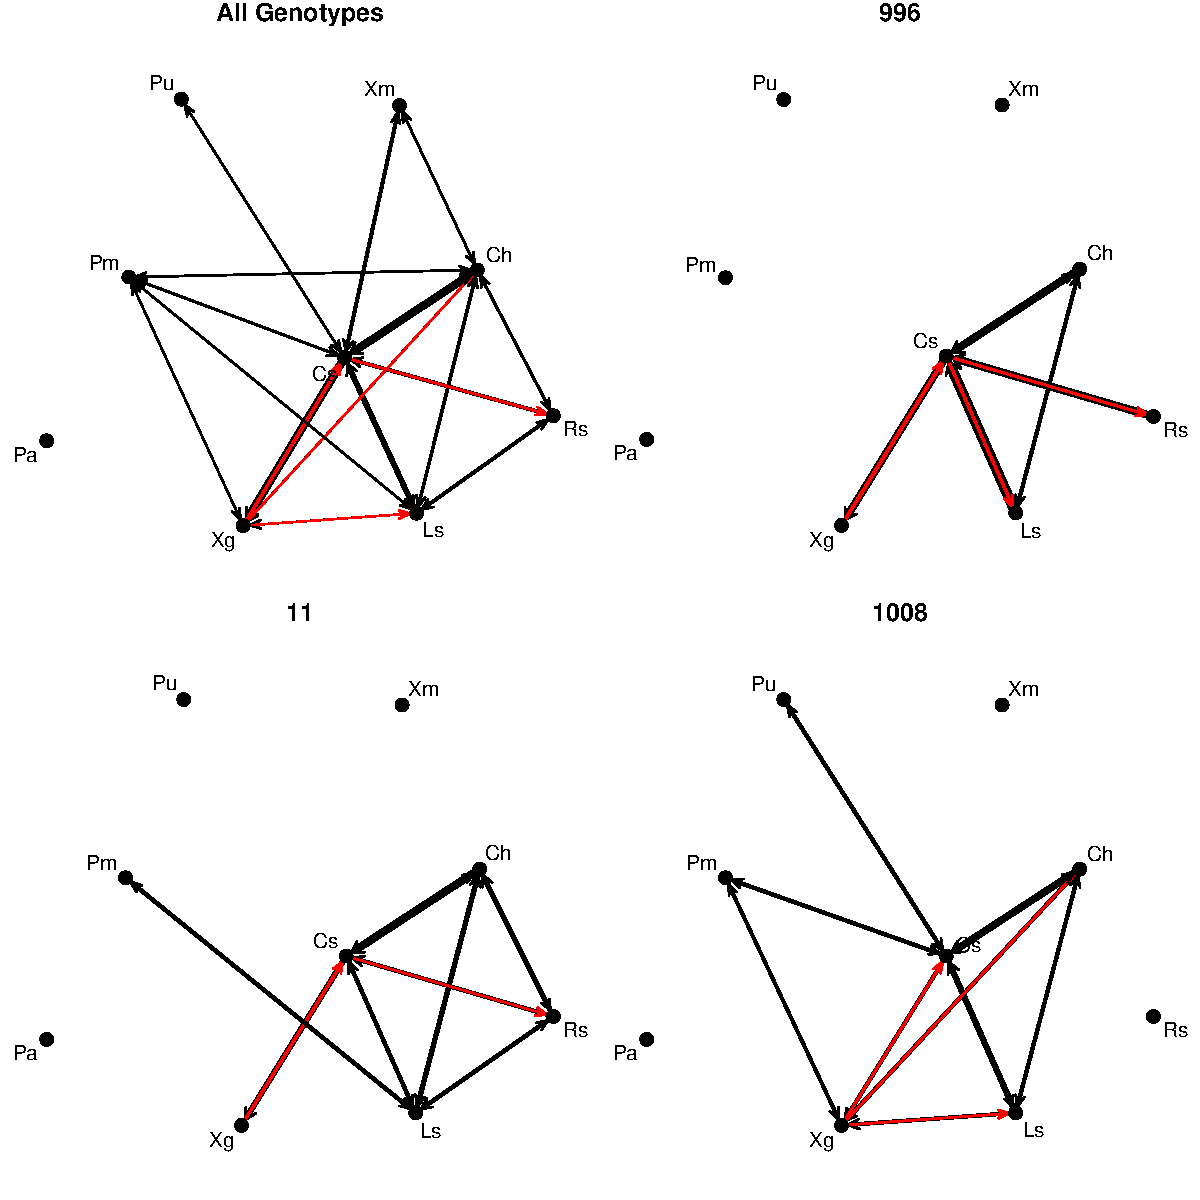
\includegraphics[width=\linewidth]{cn_onc.pdf}
\caption{Lichen networks varied in structure among genotypes. Network
  diagrams of the mean lichen interaction matrices (i.e. $\mathbf{D}$)
  averaged for all trees and for several individual genotypes showing
  a range of interaction network structure. Directionality
  (arrowheads) and sign (red = negative, black = positive) of
  interactions are shown as edges between species (abbreviated by the
  first letter of the genus and specific epithet), which are scaled by
  their magnitude.}
\label{fig:geno_nets}
\end{figure}


We observed significant lichen network structure. This structure
varied among genotypes (Fig.~\ref{fig:geno_nets}) and lichen species
varied in their importance in the network. \textit{Candaleriella
  subdeflexa} was generally the most central species (i.e. being the
most highly connected) having the highest average centrality (0.73),
followed by \textit{Ca. holocarpa} (0.54) and \textit{L. hageni}
(0.40). The centralization of the remaining species were \textit{R.}
sp. (0.18), \textit{X. galericulata} (0.14), \textit{P. melanchra}
(0.08), \textit{X. montana} (0.06) and \textit{Ph. undulata}
(0.02). \textit{Physcia adscendens} was generally not connected to
other species in the networks and had a centralization score of
zero. Interactions tended to be positive (QUANTIFY!!!); however,
\textit{X. galericulata}, although not the most central species,
frequently tended to decrease the presence of other species. 

\begin{figure}[ht]
\centering
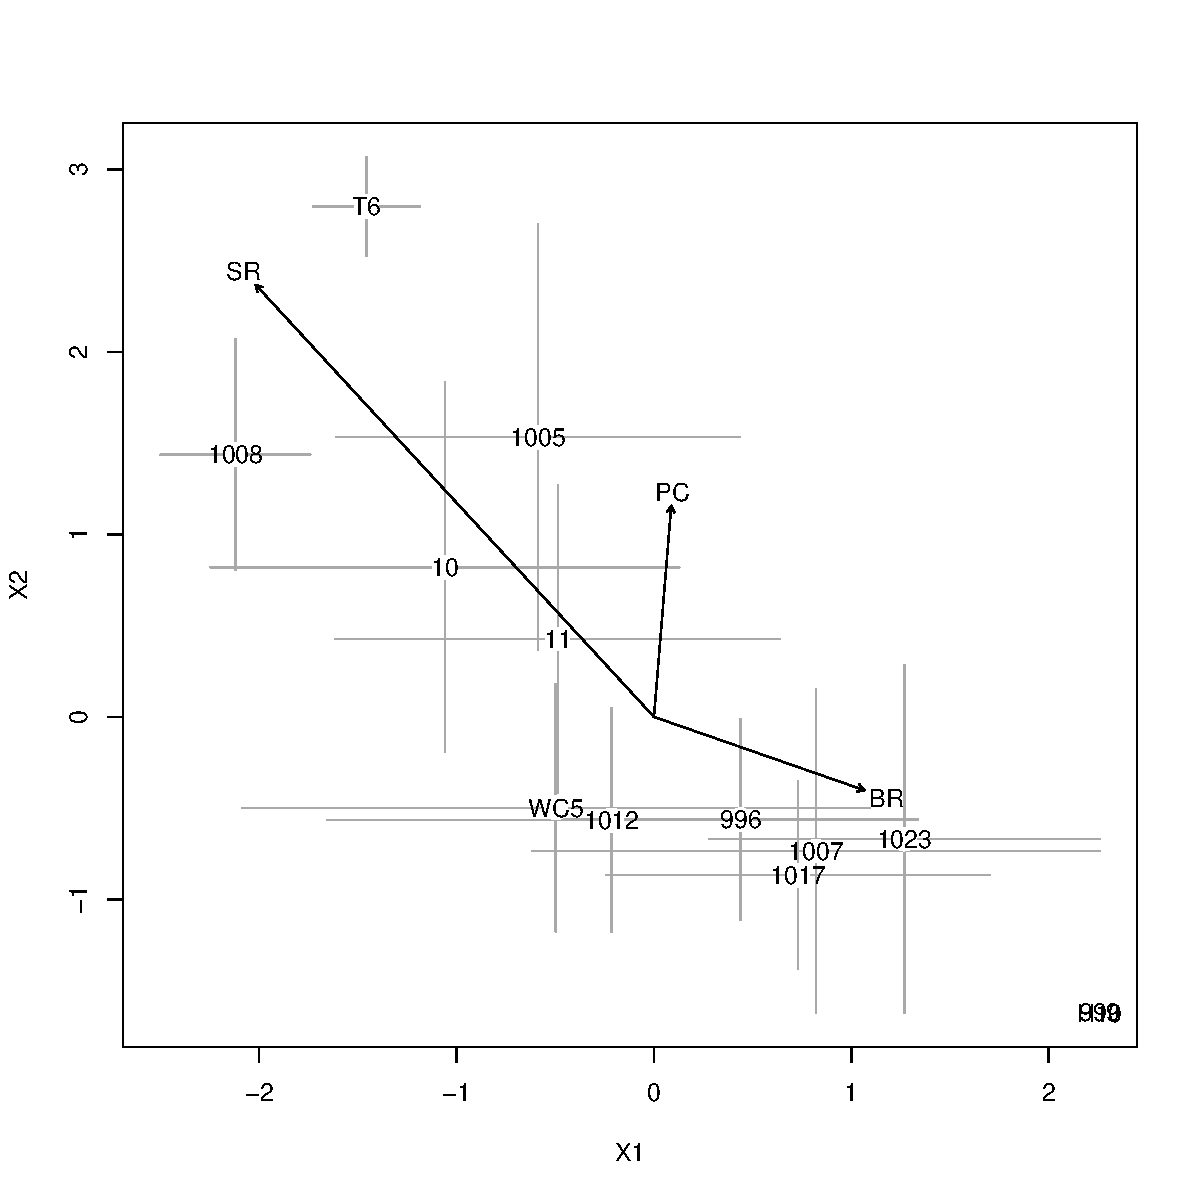
\includegraphics[width=\linewidth]{cn_chplot.pdf}
\caption{Significant lichen interaction network structure resulting
  from tree genotypic variation was observed in the common garden.
  The plot shows genotype centroids of NMDS ordinated lichen networks
  ($\pm$ 1 S.E.). Centroids that are closer are more similar in the
  structure of their lichen networks. Arrows show the magnitude and
  direction of correlation of the ordinated networks with tree bark
  roughness (BR), percent cover of lichens (PC) and lichen species
  richness (SR).}
\label{fig:cn_ch_plot}
\end{figure}


Lichen networks observed on trees of the same genotype tended to be
similar in structure. Tree genotype significantly predicted the
similarity of lichen interaction networks (PerMANOVA $R^2$ = 0.33795,
F 12 = 2.5379, p-value = 0.0050). Lichen species richness was also a
significant predictor of network similarity after controlling for
genotype (PerMANOVA $R^2$ = 0.3413, F 1 = 2.5417, p-value = 0.007399);
however, neither total cover (PerMANOVA $R^2$ = 0.023, F 1 = 2.0628,
p-value = 0.1487) nor roughness (PerMANOVA $R^2$ = 0.011, F 1 =
0.0497, p-value = 0.3394) predicted network similiarity
(Fig.~\ref{fig:cn_ch_plot}). Community similiarty was not correlated
with network similiarity (Mantel Rho spearman = 0.012, p-value =
0.337).


\begin{figure}[ht]
\centering
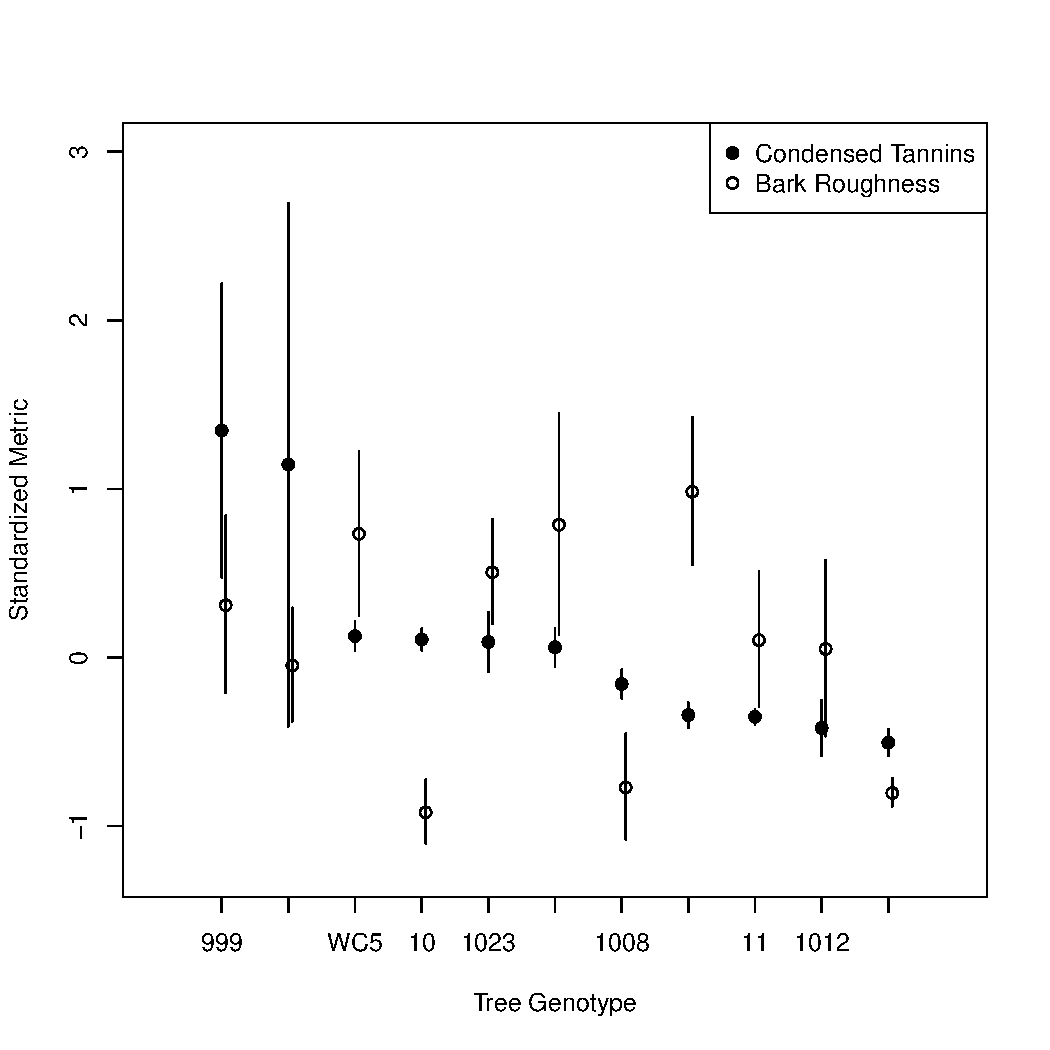
\includegraphics[width=\linewidth]{cn_metrics.pdf}
\caption{The impact of tree genotype on lichen network structure was
  indicative of variation in both the number variation in lichen
  interactions among species. This Cleveleand plot shows the means
  ($\pm$ 1 S.E.) for lichen network metrics (number of links and
  centralization) for each genotype. Both metrics are presented as
  standardized scores ($\frac{x - \bar{x}}{\sigma}$).}
\label{fig:cn_metrics}
\end{figure}


These patterns of structural similarity among networks on similar
genotypes could be partially explained by several networks. Tree
genotype marginally predicted the number of links (REML RLRT = 2.0221,
p-value = 0.0657) and centrality (REML RLRT = 2.0915, p-value =
0.0627) of lichen networks (Fig.~\ref{}). Total cover was correlated with the number
of links (ANOVA F 1 = 6.867, p-value = 0.0114) and centrality (ANOVA F
1 = 8.093, p-value = 0.0063). Lichen species richness was also
correlated with the number of links (ANOVA F 1 = 29.436, p-value =
1.46e-06) and centrality (ANOVA F 1 = 39.488, p-value =
6.38e-08). Bark roughness, however, did not significantly predict the
number of links (ANOVA F 1 = 2.897, p-value = 0.0946) nor the
centrality (ANOVA F 1 = 2.591, p-value = 0.1134) of lichen networks.
The number of network links (PerMANOVA $R^2$ = 0.392, F 1 = 72.4348,
p-value = 0.001) and network centrality (PerMANOVA $R^2$ = 0.309, F 1 =
57.0440, p-value = 0.001) were highly correlated with network
similarity.



%% % latex table generated in R 3.5.1 by xtable 1.8-3 package
%% % Thu Jan 17 20:13:56 2019
%% \begin{table}[ht]
%% \centering
%% \begin{tabular}{llll}
%%   \hline
%% Response & H2 & $R^2$ & p-value \\ 
%%   \hline
%%   Percent Rough Bark           & 0.37835 & 0.37835 & 4e-04 \\ 
%%   Lichen Network               & 0.2784  & 0.3413  & 0.0074 \\ 
%%   Percent Lichen Cover         & 0.17279 & 0.17279 & 0.0362 \\ 
%%   Number of Network Links      & 0.16892 & 0.16892 & 0.0689 \\ 
%%   Network Centrality           & 0.17248 & 0.17248 & 0.0627 \\ 
%%   Lichen Community Composition & 0.08526 & 0.27703 & 0.09529 \\ 
%%   Network Modularity           & 0.04511 & 0.04511 & 0.2941 \\ 
%%   Lichen Species Richness      & 0.03578 & 0.03578 & 0.3137 \\ 
%%    \hline
%% \end{tabular}
%% \caption{Genotypic effects of cottonwood trees on the associated lichen community.} 
%% \label{tab:h2_table}
%% \end{table}

Supplementary: Stats tables


%% Not sure if these results should be included, it might be enough to
%% just tell the unipartite network story.
%% \subsection*{Genotypic variation increases stand-level lichen network modularity}
%% \begin{itemize}
%% \item Lichens displayed signficant bipartite network structure
%% \item Bipratite network structure was greater than compared to the
%%   modularity based on a null model that randomizes with respect to genotype
%% \item z = 856.05271, p-value <= 0.00100 
%% \end{itemize}


%% In addition to including your tables within this manuscript file, PNAS
%% requires that each table be uploaded to the submission separately as a
%% “Table” file.  Please ensure that each table .tex file contains a
%% preamble, the \verb|\begin{document}| command, and the
%% \verb|\end{document}| command. This is necessary so that the
%% submission system can convert each file to PDF.


% latex table generated in R 3.4.4 by xtable 1.8-2 package
% Tue Nov 13 15:56:44 2018
\begin{table}[ht]
\centering
\begin{tabular}{llll}
  \hline
Response & Predictor & p-value & H2 \\ 
  \hline
Percent Lichen Cover & Tree Genotype & 0.0356 & 0.17 \\ 
  Lichen Species Richness & Tree Genotype & 0.1443 & 0.1 \\ 
  Percent Rough Bark & Tree Genotype & 8e-04 & 0.38 \\ 
  Lichen Network & Genotype & 0.0431 & 0.17 \\ 
  Number of Network Links & Genotype & 0.0796 & 0.15 \\ 
  Network Centrality & Genotype & 0.1351 & 0.12 \\ 
   &  &  &  \\ 
   &  &  &  \\ 
   &  &  &  \\ 
   \hline
\end{tabular}
\caption{Genotypic effects of cottonwood trees on the associated lichen community.} 
\label{tab:h2_table}
\end{table}


%% \begin{figure}
%% \centering
%% 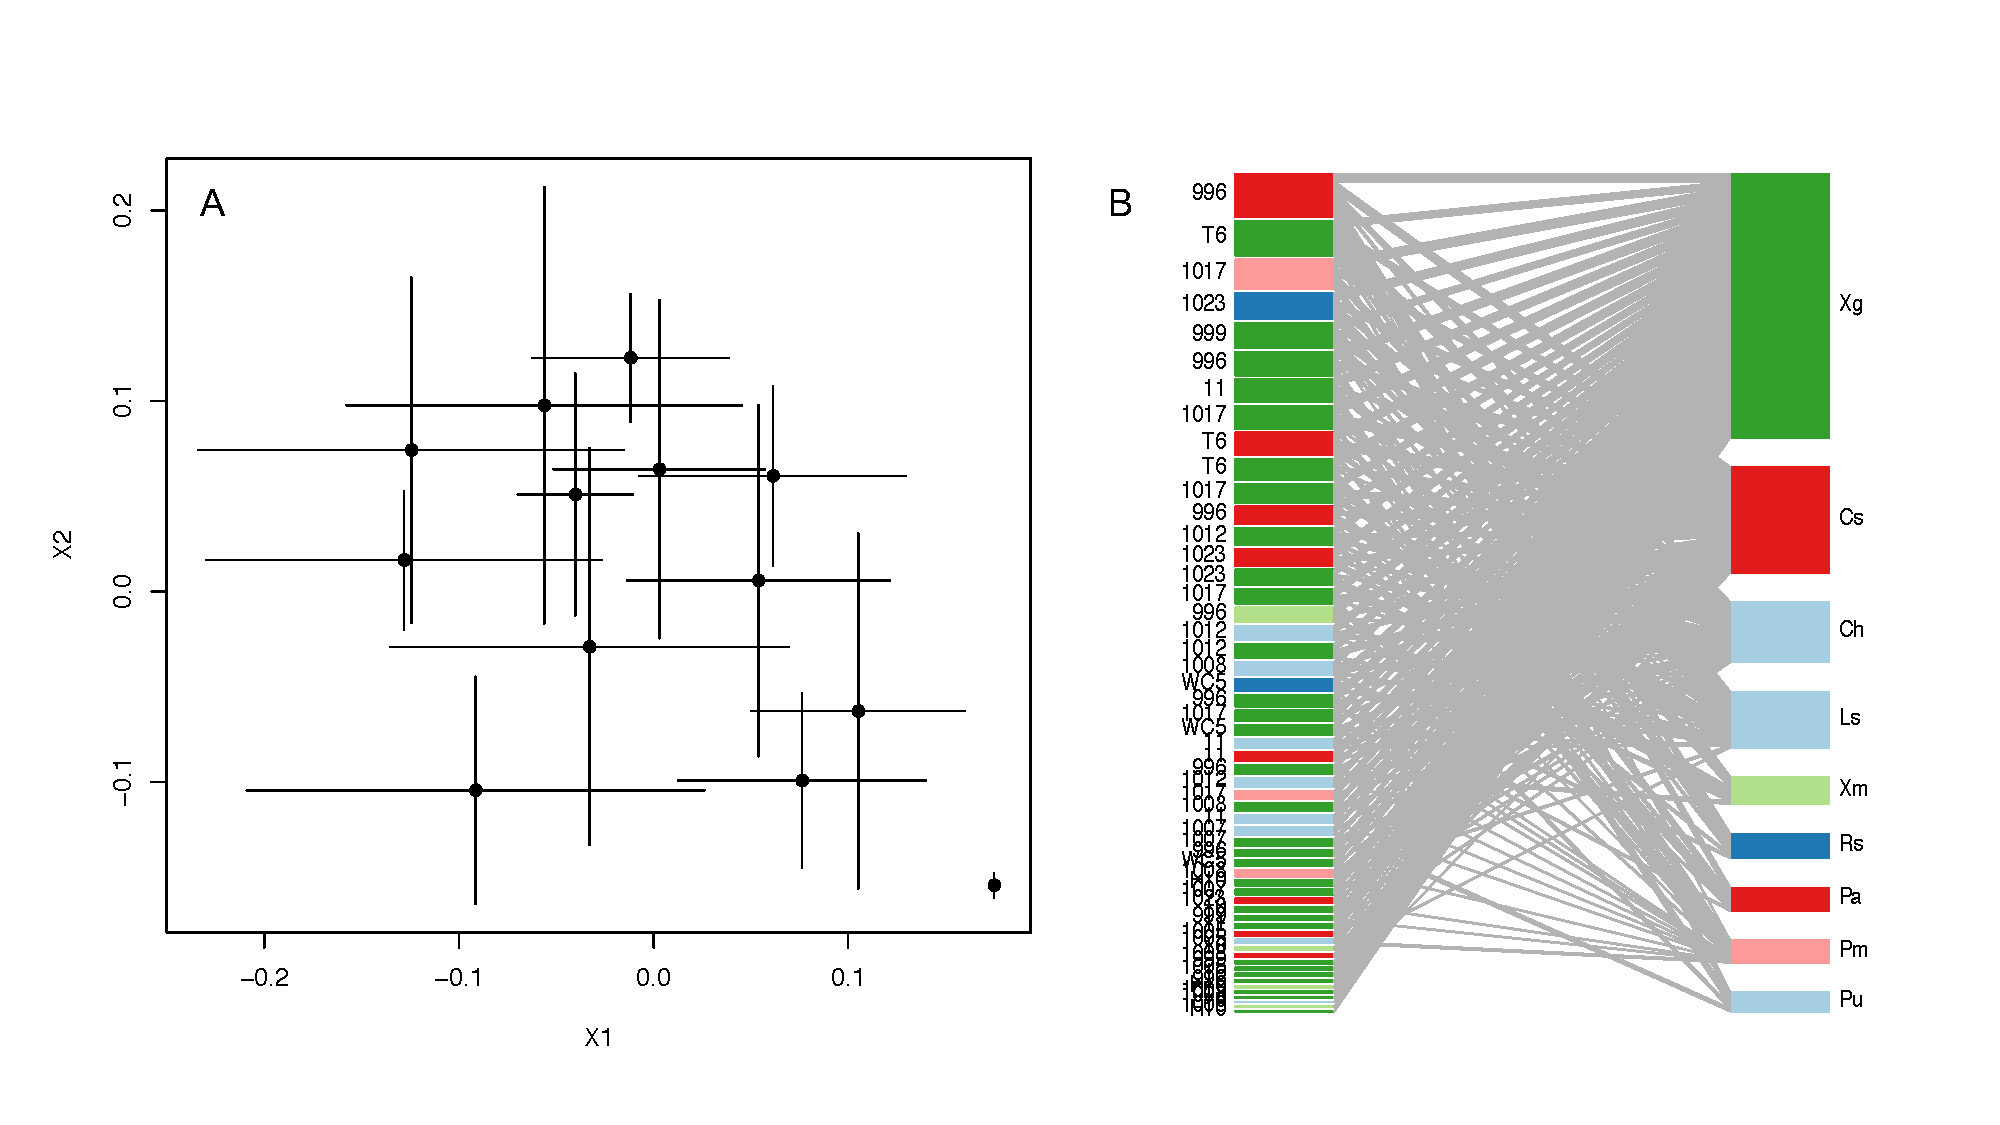
\includegraphics[width = \textwidth]{lcn_com_bpnet.pdf}
%% %% 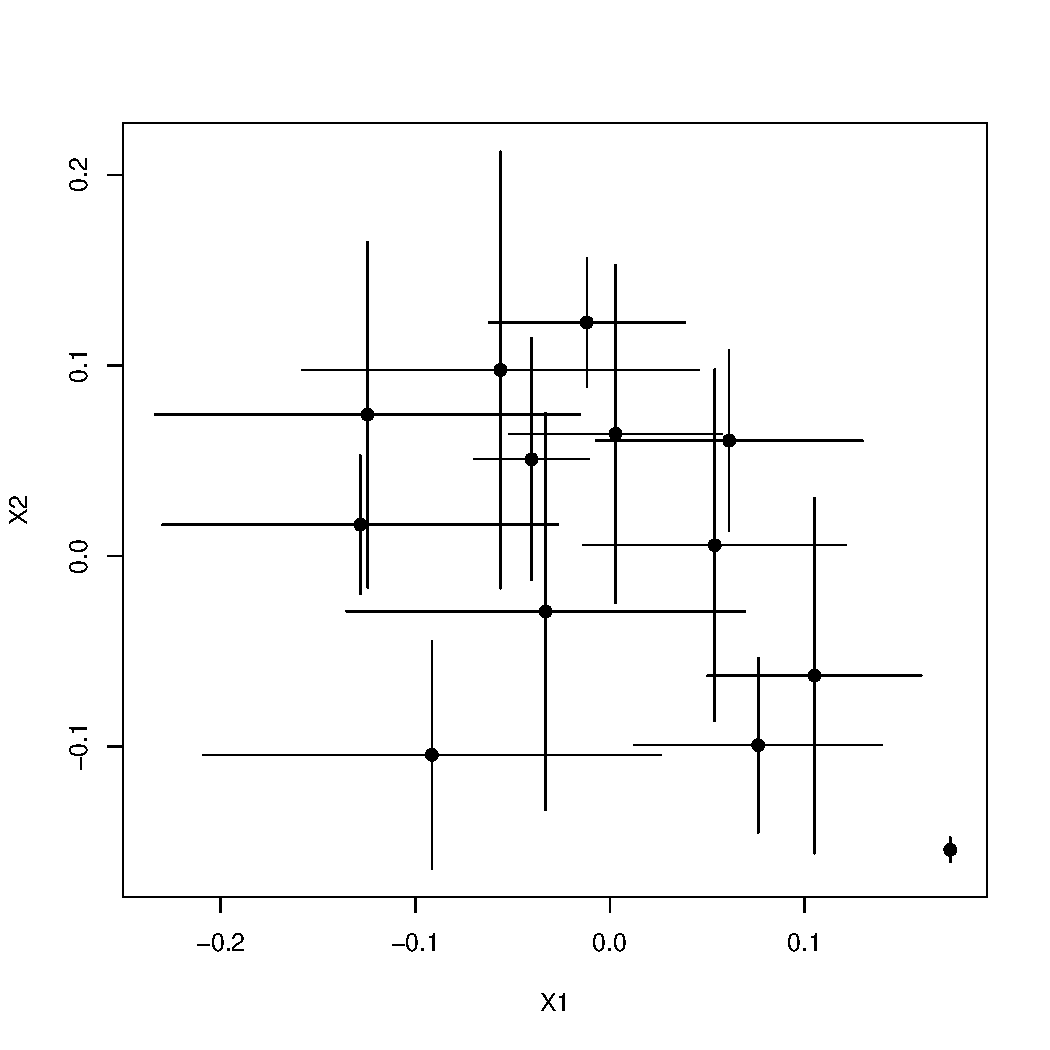
\includegraphics[width = 0.4\textwidth]{chp_com_onc.pdf}
%% %% 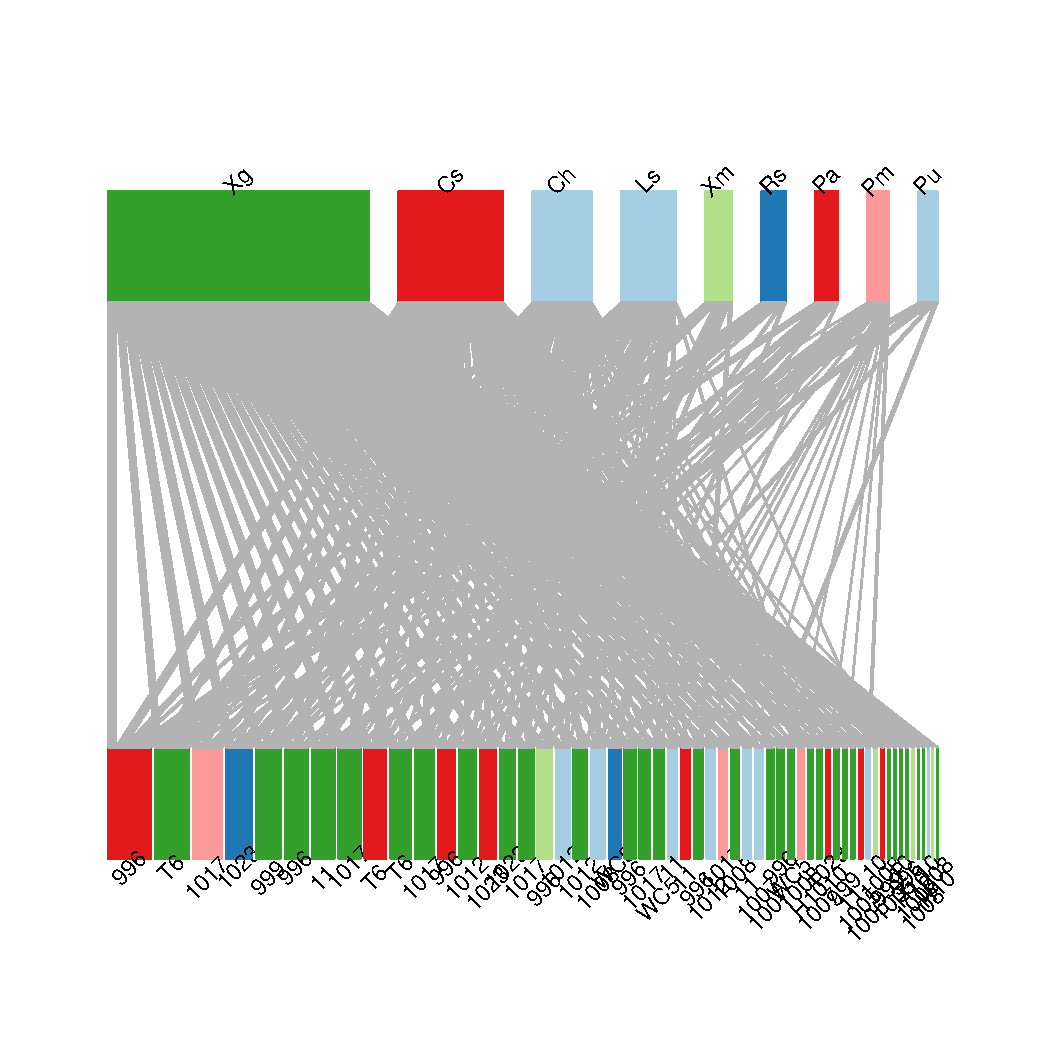
\includegraphics[width = 0.4\textwidth, angle = -90]{bp_net_onc.pdf}
%% \caption{Tree genotype varition in lichen community composition also
%%   contributed to genotype-species bipartite intreraction network
%%   structure at the scale of the common garden stand. A) Plot of the
%%   ordinated community composition scores shown as centroids ($\pm$ 1
%%   S.E.). B) Bipartite interaction network based on the occurrences of
%%   lichen on individual cottonwood trees in the common garden. Edges
%%   connecting trees to lichen are scaled by the relative abundance of
%%   lichen. Nodes of lichen and trees are colored by their module
%%   membership.}
%% \label{fig:bpnet}
%% \end{figure}




}


\showmatmethods{} % Display the Materials and Methods section


\section*{Discussion}

\begin{itemize}
\item Rehash of results support hypothesis of genetic basis to network structure
\item Genotypic environmental filtering leads to altered interaction
  network structure and potentially dymanics
\item Indirect effects of genotypes (G - rough - cover - richness -
  links - networks)
\item Importance of indirect effects and complexity and releveance to IIGEs
\item Conclusion
\end{itemize}



Trait variation + assembly + ecosystem function

These findings support the hypothesis that genotypic variation in a
foundation species contributes to the structure of a network of
interacting species that might be least expected to exhibit such
structure. 

\textbf{TGW: MIGHT BE GOOD TO CITE PAPERS ON COMEPTITION IN LICHENS OR
OTHER ORGANIZING FACTORS TO BACK UP THE LEAST EXPECTED STATEMENT.  AS
EPIPHYTES WE MIGHT NOT EXPECT THEM TO CARE.}

\textbf{MKL: This is a job for Lamit and Rikke.}

Several lines of evidence support this conclusion. First, the wild
stand showed significant interaction network structure (Fig. 1a and
b); and both tree genotype and the genetically based tree trait, bark
roughness, was a strong predictor of co-occurrence patterns
(Fig. 2a). 

\textbf{TGW: I THINK WE NEED TO EMPHASIZE THE LONG-TERM NATURE OF OUR
COMMON GARDEN STUDY AS VERY FEW COMMON GARDEN STUDIES OF LICHENS
LIKELY EXIST. ANY REFS ON THIS? IF TRUE MIGHT WANT TO MENTION THIS UP
FRONT IN INTRO.}

\textbf{MKL: Same here. This is a job for Lamit and Rikke.}

Second, in a long-term common garden study, network
(Fig. 1b) structure showed a high degree of similarity to the wild
stand network structure (Fig. 1c and d). Third, tree genotype was a
significant predictor of SES values (Fig. 2a), displaying significant
correlation with a genetically linked trait, bark roughness, both in
the common garden (Fig. 2a) and in a naturally established stand of
trees (Fig. 2b). Last, both of the bipartite genotype-species networks
in the common garden and natural stand displayed significant
modularity, suggesting that genotypic variation is leading to the
formation of evolutionarily dynamic compartments within the
community. Thus, just as numerous studies have shown that plant
genotype can affect species richness, abundance, diversity, and
composition and previous work has demonstrated that evolutionary
processes shape ecological networks \cite{Guimaraes2011,
  Moya-Larano2011}, our study includes genetics in an empirical
investigation that combines both experimental common garden findings
along with studies in the wild that are in close agreement.

Our results point to the importance of understanding the community
level effects of genetic variation and corroborate previous findings
of the importance of plant genetics in shaping community structure and
ecosystem processes \cite{Whitham2006a}.  This study highlights the
potential for indirect effects of genetic variation to propagate
through networks of interacting species and trophic levels. Altering
the structure of interaction networks presents a means for genetic
effects to be magnified within the system of interacting species. For
example, Keith et al. (2017) showed that the genetics based
interations of aphid resistant and aphid susceptible trees resulted in
different interaction networks of their associated arthropod
communities composed of 139 species. At the scale of ecosystems,
trophic networks or food webs direct and control the rates of energy
and nutrient flux \cite{Borgatti2006}. Furthermore, in a
predator-prey-plant study, Smith \cite{Smith2011}, showed that the
interactions among species across trophic levels depended on plant
genotype.

\subsection{Units of evolutionary potential: Moving beyond species pairs}


Although our study was conducted with a community of lichens, these
results should be generalized to other groups of diverse organisms
around the world that also exhibit significant genetic signals at the
community level \cite{Rowntree2011, Whitham2012}, although spatial
scale of interactions should be considered \cite{Zook2010} Bangert et
al. 2006. As heritable variation is the raw material for natural
selection to act upon, a genetic basis for interaction network
structure indicates evolutionary dynamics should be considered at the
community level and that conserving genetic variation is important to
consider in efforts to restore or preserve complex species
interactions and their associated ecosystem functions
\cite{Evans2013}.  With such findings, it appears that we are closer
to understanding the evolutionary drivers of Darwin's entangled bank
and the interconnectedness of species in complex communities.

%% Please include your acknowledgments here, set in a single
%% paragraph. Please do not include any acknowledgments in the
%% Supporting Information, or anywhere else in the manuscript.

\acknow{This work was supported by the National Science Foundation grant
(DEB-0425908) and Integrative Graduate Research Traineeship (IGERT)
fellowships for M.L. and L.L. The Ogden Nature Center staff helped to
maintain the common gardens. Lichen sampling was supported by Todd
Wojtowicz, Luke Evans and David Solance Smith.}

\showacknow{} % Display the acknowledgments section

\bibliography{lichen_network_genetics}

\end{document}

%% \subsection*{Supporting Information (SI)}

%% Authors should submit SI as a single separate PDF file, combining
%% all text, figures, tables, movie legends, and SI references.  PNAS
%% will publish SI uncomposed, as the authors have provided it.
%% Additional details can be found here:
%% \href{http://www.pnas.org/page/authors/journal-policies}{policy on
%% SI}.  For SI formatting instructions click
%% \href{https://www.pnascentral.org/cgi-bin/main.plex?form_type=display_auth_si_instructions}{here}.
%% The PNAS Overleaf SI template can be found
%% \href{https://www.overleaf.com/latex/templates/pnas-template-for-supplementary-information/wqfsfqwyjtsd}{here}.
%% Refer to the SI Appendix in the manuscript at an appropriate point
%% in the text. Number supporting figures and tables starting with S1,
%% S2, etc.

%% Authors who place detailed materials and methods in an SI Appendix
%% must provide sufficient detail in the main text methods to enable a
%% reader to follow the logic of the procedures and results and also
%% must reference the SI methods. If a paper is fundamentally a study
%% of a new method or technique, then the methods must be described
%% completely in the main text.

%% \subsubsection*{SI Datasets} 

%% Supply Excel (.xls), RTF, or PDF files. This file type will be
%% published in raw format and will not be edited or composed.

%% \subsubsection*{SI Movies}

%% Supply Audio Video Interleave (avi), Quicktime (mov), Windows Media
%% (wmv), animated GIF (gif), or MPEG files and submit a brief legend
%% for each movie in a Word or RTF file. All movies should be
%% submitted at the desired reproduction size and length. Movies
%% should be no more than 10 MB in size.


%% \subsubsection*{3D Figures}

%% Supply a composable U3D or PRC file so that it may be edited and
%% composed. Authors may submit a PDF file but please note it will be
%% published in raw format and will not be edited or composed.

